\section{Clinical applicability}

\begin{frame}[plain,c]
    %\frametitle{A first slide}

    \begin{center}
        \color{DarkBlue}
    \Huge \thesection. \insertsection
    \end{center}

\end{frame}


\begin{frame}{Learnlets - 1~[Ramzi et al. 2021a]}
    % show the generalization figure
    \begin{exampleblock}{Contribution \#4}
        \fullcite{Ramzi2021WaveletsEra}
    \end{exampleblock}
    \begin{figure}
        \centering
        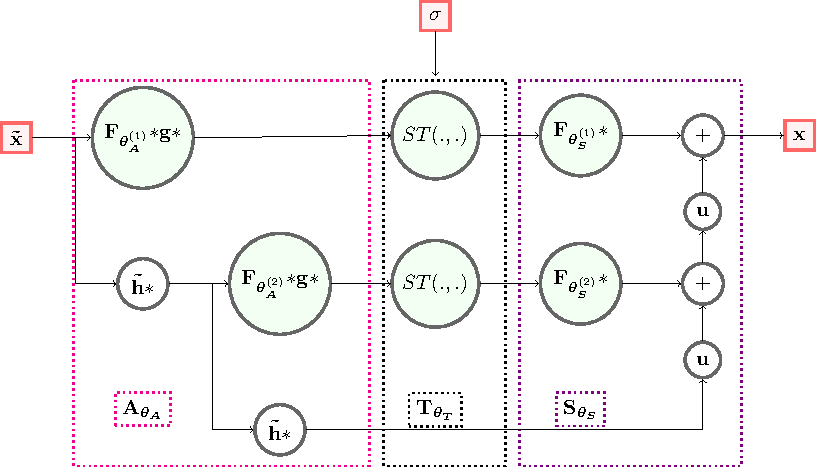
\includegraphics[height=0.53\textheight]{Figures/clinic_applic/learnlets_tikz_reduced.pdf}
    \end{figure}
    \let\thefootnote\relax\footnotetext{
        ST: Soft Thresholding
    }
\end{frame}

\begin{frame}{Learnlets - 2~[Ramzi et al. 2021a]}
    % show the generalization figure
    \begin{figure}[ht]
        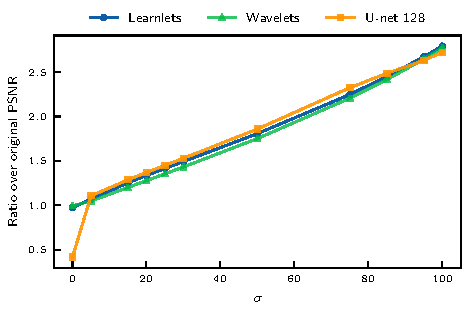
\includegraphics[height=0.78\textheight]{Figures/clinic_applic/model_comparison.pdf}
        \caption{\textbf{Denoising performances.}}
        \end{figure}
\end{frame}

\begin{frame}{Denoising Score Matching - 1~[Ramzi et al. 2020d]}
    % show the samples
    \begin{exampleblock}{Contribution \#5}
        \fullcite{Ramzi2020_dsm}
    \end{exampleblock}
    Optimal denoiser:\footfullcite{Vincent2011,Alain2013}
    \begin{equation*}
        \rb^\star(\xb', \sigma) = \xb' + \sigma^2 \nabla_{\xb} \log p_{\sigma^2}(\xb')
    \end{equation*}
    where $p_{\sigma^2} = p \ast \mathcal{N}(0, \sigma^2)$.
\end{frame}

\begin{frame}{Denoising Score Matching - 2~[Ramzi et al. 2020d]}
    % show the samples
    \begin{figure}
        \centering
        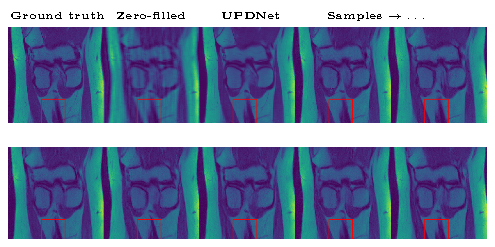
\includegraphics[width=\textwidth]{Figures/clinic_applic/dsm_main.pdf}
    \end{figure}

\end{frame}
